\documentclass[11pt,a4paper]{article}
\usepackage[margin=1in]{geometry}
\usepackage[T1]{fontenc}
\usepackage{enumitem}
\usepackage{titlesec}
\usepackage{parskip}
\usepackage{setspace}
\usepackage{array}
\usepackage{tikz}
\usetikzlibrary{arrows.meta,fit,backgrounds}
\setstretch{1.05}

\pagestyle{empty}
\setlist{itemsep=0.2em,topsep=0.3em,leftmargin=1.5em}
\titleformat{\section}{\large\bfseries}{\thesection.}{0.5em}{}
\titlespacing*{\section}{0pt}{1.2em}{0.4em}

\newcolumntype{L}[1]{>{\raggedright\arraybackslash}p{#1}}

\begin{document}

\noindent\textbf{Terminal Touchers}\hfill\textbf{Megathon X: M1 Approach}

\vspace{0.3em}
\begin{center}
{\LARGE\bfseries Green Customer Insights Platform}
\end{center}
\vspace{-0.3em}
\hrule

\section{Problem Understanding}
Lloyds wants a platform that reads a customer's transactions, holdings and behaviour and works out which green products might suit them, roughly how much CO$_2$e that would save, and why. Four products are mandatory (EV Finance, Green Home Loan, Solar Finance, Paperless Banking). Green Investments and Green Loans are optional.

Most of our design follows from the brief's rule that every component does one job only:
\begin{itemize}
  \item \textbf{One job per component.} The ML models predict take-up propensity and nothing else. Carbon impact comes from a rules-based engine using published emission factors. Eligibility comes from product rules. The LLM only rewrites structured records into plain English; it never predicts, calculates or decides.
  \item \textbf{Propensity is not eligibility.} A high score for a customer who fails the product rules still gets no offer. Redundant offers are blocked outright, such as EV finance for someone who already owns an EV.
  \item \textbf{Every recommendation can be explained.} Each one carries evidence, a confidence value, fixed reason codes and a data timestamp.
\end{itemize}

\section{Idea in Brief}
We are building a pipeline in five steps. It joins transactions, demographics and holdings into one Customer 360 record per customer, and sorts every transaction into exactly one of eight categories (Fuel, Electricity, Gas, Public Transport, Home Improvement, Automotive, Utilities, Other). A classifier then scores each customer against each product. Separately, a carbon engine estimates annual CO$_2$e savings with documented formulas. A guardrail layer removes anything the customer is ineligible for or already has. Whatever survives goes to an LLM, which writes the customer-facing text, and into a Streamlit dashboard for relationship managers.

\section{Data Sources and Augmentation}
The brief rules out real banking data, and no single public dataset has transactions, holdings and take-up labels together. So we are combining public sources and then generating the missing parts. Public sources set the shape and realism of the data, and synthetic generation fills in the rest.

\begin{center}
\footnotesize
\renewcommand{\arraystretch}{1.15}
\begin{tabular}{|L{4.6cm}|L{6.4cm}|L{3.4cm}|}
\hline
\textbf{Source} & \textbf{What we take from it} & \textbf{Used for} \\ \hline
Sparkov synthetic card-transaction data (Kaggle release) & Merchant names, merchant categories, amounts, timestamps, geography & Base transaction table \\ \hline
UK transaction sample (Mendeley Data, \texttt{dnxtg6n4rv}, about 6.5k records) & UK-style merchant descriptions and amounts & Testing and tuning the categoriser on UK merchant strings \\ \hline
ONS ``Revolut spending on debit cards'' (weekly and monthly indices) & Index series of UK debit card spend over time & Seasonality and trend shape for monthly spend; not customer-level \\ \hline
DESNZ NEED anonymised data 2025 (50k-row sample) & Annual gas and electricity use (2005--2023), property type, age, floor area, region, EPC band, installed efficiency measures & Home profile and energy use for each synthetic customer \\ \hline
UCI Bank Marketing dataset (Moro et al., 2014) & How age, job, balance and prior contact relate to product take-up & Template for label structure \\ \hline
ONS Family Spending (Living Costs and Food Survey) & Household spend by category and income band & Calibrating spend levels \\ \hline
DfT National Travel Survey & Annual car mileage by region and household type & Mileage distribution \\ \hline
DfT/DVLA vehicle licensing statistics & Share of EV and petrol/diesel cars by region & Ownership priors \\ \hline
Ofgem typical domestic consumption values & Typical household kWh for electricity and gas & Spend-to-kWh conversion \\ \hline
EPC open data (MHCLG) & Property type, tenure, EPC band, heating type, solar PV flag & Home attributes for Green Home and Solar \\ \hline
MCS installation statistics & Solar installs by area & Regional solar priors \\ \hline
ISO 18245 merchant category codes & Code-to-merchant-type mapping & Seeding categoriser rules \\ \hline
DESNZ/DEFRA GHG conversion factors; National Grid ESO Carbon Intensity data & kgCO$_2$e per km, litre, kWh and kg of paper; grid intensity & Carbon engine \\ \hline
\end{tabular}
\end{center}

\textbf{How we augment.} We start from the Sparkov transactions and remap their merchant types onto our eight categories. Around 50,000 customers with twelve months of history is our target. Profile and holdings tables (age, income band, tenure, region, loans, vehicle, solar, statement preference) are generated with Faker and the Synthetic Data Vault, sampling from marginals taken from the ONS and DfT sources above. For the home side, each synthetic customer is paired with a real record from the 50k NEED sample, so property type, floor area, region, EPC band and gas and electricity use come from actual English and Welsh homes. Electricity and gas bills in the transaction table are then derived from that consumption, which keeps the Solar and Green Home signals consistent with the property. The Revolut index series only shapes month-to-month seasonality in spend, since it has no customer-level rows. Spend is then rescaled so each customer's totals are consistent with their income band and region. We also add recurring fuel, energy-supplier and home-improvement transactions, since the base data has few of these.

\textbf{How we label.} Take-up labels are not random. For each customer and product we compute a latent score from the features that should plausibly drive it (e.g.\ fuel share and mileage for EV Finance, electricity spend and home ownership for Solar), add noise, and sample a Bernoulli outcome. Coefficients, noise level and the hard exclusion rules are all written down in the repo. A known weakness is that the models are learning our own generator, so held-out scores will look better than real-world performance would. We will say so in the evaluation report, and we will also test on a second dataset generated with different coefficients and seed.


\section{Product Signals and Guardrails}
These are the rules we plan to start from. Thresholds will be tuned once we see the generated data. We do not have Lloyds' actual authorised product rules, so the eligibility checks are stand-ins (age 18+, not in arrears, basic affordability) and are kept in a separate config file so they can be swapped out.

\begin{center}
\small
\begin{tabular}{|L{3.0cm}|L{5.6cm}|L{6.0cm}|}
\hline
\textbf{Product} & \textbf{Signals (model input)} & \textbf{Negative guardrail} \\ \hline
EV Finance & Fuel and Automotive spend, mileage estimate, public transport use, income band & Already owns an EV; no replacement use case \\ \hline
Green Home Loan & Home Improvement spend, utility bills, EPC band, mortgage or ownership & Existing green home loan; fails eligibility rules \\ \hline
Solar Finance & High electricity spend, owner-occupier, property type & Already has solar finance; not a homeowner \\ \hline
Paperless Banking & Share of digital transactions, app logins & Already paperless \\ \hline
\end{tabular}
\end{center}

\textbf{Category boundaries.} Categories are mutually exclusive, so the edge cases need fixed rules. Pump purchases are Fuel, while servicing, parts, MOT, parking and car washes are Automotive. Named energy suppliers go to Electricity or Gas, while water, broadband and council tax go to Utilities. A dual-fuel bill cannot be split, so it goes to Electricity unless the description says gas. Merchant matching uses keyword and regex rules seeded from the MCC list, with a small TF-IDF fallback model for merchants the rules miss. The Mendeley UK sample is our check that the rules still work on UK-style merchant strings, not just the Sparkov names.

\section{Architecture}
Figure~1 shows the flow. The three boxes in the dashed group run side by side on the same Customer 360 table. Their outputs meet at the recommendation engine, which is the only place a customer-product pair is accepted or rejected.

\begin{figure}[h]
\centering
\resizebox{\textwidth}{!}{%
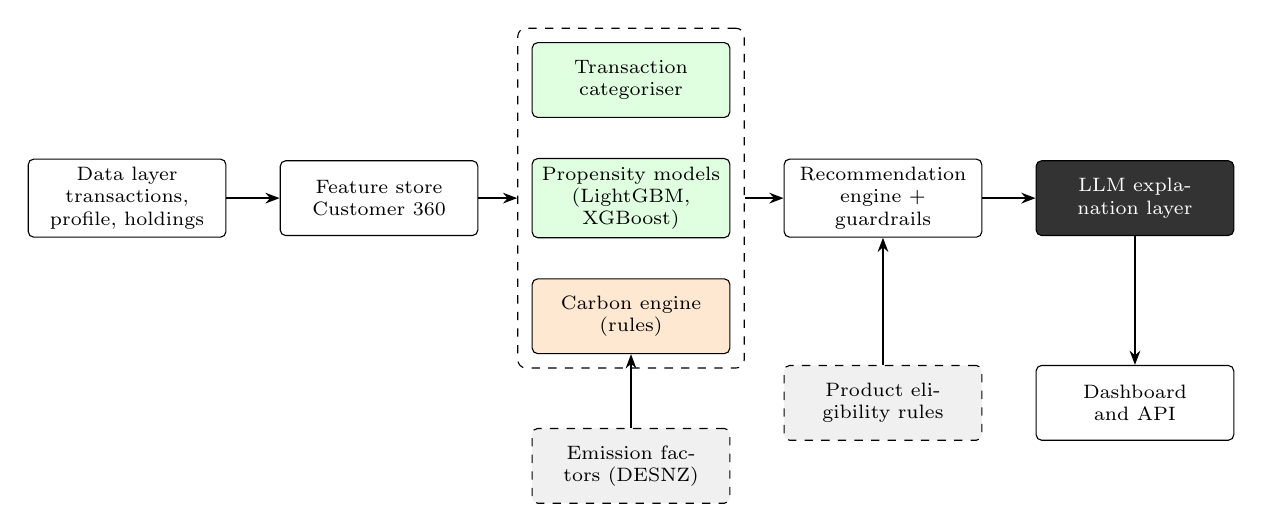
\begin{tikzpicture}[
  box/.style={draw, rounded corners=2pt, align=center, font=\scriptsize, text width=2.3cm, minimum height=0.95cm, inner sep=3pt, fill=white},
  ext/.style={box, dashed, fill=gray!12},
  llm/.style={box, fill=black!80, text=white},
  arr/.style={-{Stealth[length=1.8mm]}, thick}
]
\node[box] (data) at (0,0) {Data layer\\ transactions, profile, holdings};
\node[box] (fs) at (3.2,0) {Feature store\\ Customer 360};
\node[box, fill=green!12] (cat) at (6.4,1.5) {Transaction categoriser};
\node[box, fill=green!12] (ml) at (6.4,0) {Propensity models\\ (LightGBM, XGBoost)};
\node[box, fill=orange!18] (co2) at (6.4,-1.5) {Carbon engine\\ (rules)};
\node[box] (rec) at (9.6,0) {Recommendation engine + guardrails};
\node[llm] (llm) at (12.8,0) {LLM explanation layer};
\node[box] (dash) at (12.8,-2.6) {Dashboard and API};
\node[ext] (ef) at (6.4,-3.4) {Emission factors (DESNZ)};
\node[ext] (rules) at (9.6,-2.6) {Product eligibility rules};

\begin{scope}[on background layer]
  \node[draw, dashed, rounded corners=3pt, fit=(cat)(ml)(co2), inner sep=5pt] (grp) {};
\end{scope}

\draw[arr] (data) -- (fs);
\draw[arr] (fs) -- (grp);
\draw[arr] (grp) -- (rec);
\draw[arr] (rec) -- (llm);
\draw[arr] (llm) -- (dash);
\draw[arr] (ef) -- (co2);
\draw[arr] (rules) -- (rec);
\end{tikzpicture}}
\par\vspace{0.4em}{\small Figure 1. Pipeline. Grey dashed boxes are static reference inputs; the dashed group runs in parallel.}
\end{figure}

\begin{enumerate}
  \item \textbf{Ingestion and feature store.} Join transactions, profile and holdings on customer ID. Splits are made at customer level (70/15/15), so no customer appears in more than one split.
  \item \textbf{Categorisation and Customer 360.} Apply the category rules, then aggregate to monthly and annual features per customer.
  \item \textbf{Propensity and carbon.} One LightGBM or XGBoost classifier per required product outputs a probability. Confidence combines how much the scores of a small bootstrap ensemble disagree with how many months of data the customer has, so sparse histories get lower confidence. Reason codes are fixed identifiers derived from the top SHAP features. The carbon engine is separate; see below.
  \item \textbf{Recommendation and guardrails.} Drop pairs that fail holdings checks or eligibility rules, then rank what is left.
  \item \textbf{Presentation.} The LLM receives one JSON record per pair and writes a short explanation. A checker confirms that every number and reason code in the text appears in the record. If it does not, we fall back to a plain template.
\end{enumerate}

\textbf{Carbon engine.} For EV Finance, annual litres are estimated from fuel spend and an average pump price, then converted to distance using a default fuel economy by vehicle class. Savings are $E_{\text{before}} - E_{\text{after}}$, where $E_{\text{before}}$ is litres times the DESNZ per-litre factor and $E_{\text{after}}$ is distance times an assumed kWh/km times the UK grid factor. Solar uses electricity spend converted to kWh, an assumed system size capped at a fraction of household use, and a fixed yield per kWp. Green Home uses EPC-band lookups for typical gas reduction after retrofit. Paperless uses an assumed number of sheets per year times a per-kg paper factor. Every factor, unit, source and base year sits in one versioned CSV that ships with the submission, and results are shown as an estimate with the assumptions noted.

\section{Testing Plan}
\begin{itemize}
  \item \textbf{Baselines.} Compare against logistic regression and against a simple rule (e.g.\ top-quartile spend in the relevant category) to see what the gradient-boosted models actually add.
  \item \textbf{Metrics.} ROC-AUC, PR-AUC and F1 on the customer-level validation and test sets, since take-up is rare. We also report Brier score and a calibration curve, because the propensity values are shown to users as probabilities.
  \item \textbf{Scenario tests.} Customers with sparse or missing months, conflicting records (e.g.\ EV owner with fuel spend), no mileage data, and customers whose circumstances change between snapshots. Existing holders must never be offered the same product.
  \item \textbf{LLM checks.} A hand-checked set of about 200 records scored for faithfulness (all numbers match) and for banned content (no eligibility claims, no invented facts).
  \item \textbf{Reproducibility.} Fixed seeds, pinned requirements, and a Docker image with a single entry point for preprocessing, training and inference.
\end{itemize}

\section{Explainable Output and Dashboard}
Each customer-product pair produces one record: product, propensity, confidence, reason codes, the spend categories and values used as evidence, estimated CO$_2$e saving, eligibility status and a data timestamp. The customer sees the explanation and a single action, such as ``Explore EV options'' or ``Go paperless''. The dashboard aggregates the same records into customers analysed, opportunities by product, estimated impact, regional trends and top segments, and lets a manager drill from segment to customer to evidence to action.

\end{document}
